%% MODELO DE LATEX PARA TRABALHOS ACADÊMICOS

\documentclass[
	% -- opções da classe memoir --
	12pt,				% tamanho da fonte
	% openright,			% capítulos começam em pág ímpar (insere página vazia caso preciso)
    oneside,			% para impressão somente frente. Oposto a twoside (frente e verso)
	a4paper,			% tamanho do papel. 
	% -- opções da classe abntex2 --
	%chapter=TITLE,		% títulos de capítulos convertidos em letras maiúsculas
	%section=TITLE,		% títulos de seções convertidos em letras maiúsculas
	%subsection=TITLE,	% títulos de subseções convertidos em letras maiúsculas
	%subsubsection=TITLE,% títulos de subsubseções convertidos em letras maiúsculas
	% -- opções do pacote babel --
	english,			% idioma adicional para hifenização
	french,				% idioma adicional para hifenização
	spanish,			% idioma adicional para hifenização
	brazil,				% o último idioma é o principal do documento
	]{abntex2}


% ---
% PACOTES
% ---

% ---
% Pacotes fundamentais 
\usepackage{longtable}
\usepackage{graphicx,url}
\usepackage{graphicx,url}
\usepackage{fourier} 
\usepackage{array}
\usepackage{makecell}
\usepackage[utf8]{inputenc}
\usepackage[brazil]{babel}
\usepackage{float}
\usepackage{footnote}
\usepackage{graphicx}
\usepackage{caption}
\usepackage{subcaption}
\usepackage{graphicx}
\usepackage[most]{tcolorbox}
\usepackage{graphicx,url}
\usepackage[export]{adjustbox}
\usepackage[utf8]{inputenc}
\usepackage[brazil]{babel}
\usepackage{float}
\usepackage{footnote}
\usepackage{graphicx}
\usepackage{array}
\usepackage[most]{tcolorbox}
\usepackage{graphicx,url}
\usepackage{booktabs,chemformula}
\usepackage[export]{adjustbox}
\usepackage{float}
\usepackage{cmap}				% Mapear caracteres especiais no PDF
\usepackage{lmodern}			% Usa a fonte Latin Modern
\usepackage[T1]{fontenc}		% Selecao de codigos de fonte.
\usepackage[utf8]{inputenc}		% Codificacao do documento (conversão automática dos acentos)
\usepackage{indentfirst}		% Indenta o primeiro parágrafo de cada seção.
\usepackage{color}				% Controle das cores
\usepackage{graphicx}			% Inclusão de gráficos
\usepackage{epigraph}
\usepackage{booktabs}
\usepackage{multicol}
\usepackage{multirow}
\usepackage{lipsum}				% para geração de dummy text
\usepackage[brazilian,hyperpageref]{backref}	 % Paginas com as citações na bibl
\usepackage[alf]{abntex2cite}	% Citações padrão ABNT
% ---
\usepackage{cmap}				% Mapear caracteres especiais no PDF
\usepackage{csquotes}
\usepackage{lmodern}			% Usa a fonte Latin Modern
\usepackage[T1]{fontenc}		% Selecao de codigos de fonte.
\usepackage[utf8]{inputenc}		% Codificacao do documento (conversão automática dos acentos)
\usepackage{indentfirst}		% Indenta o primeiro parágrafo de cada seção.
\usepackage{color}				% Controle das cores
\usepackage{graphicx}			% Inclusão de gráficos
\usepackage{epigraph}
\usepackage{multicol}
\usepackage{multirow}
\usepackage{lipsum}				% para geração de dummy text
\usepackage[brazilian,hyperpageref]{backref}	 % Paginas com as citações na bibl
\usepackage[alf]{abntex2cite}	% Citações padrão ABNT
\usepackage{float}
\usepackage{csquotes}
\usepackage{cmap}				% Mapear caracteres especiais no PDF
\usepackage{lmodern}			% Usa a fonte Latin Modern
\usepackage[T1]{fontenc}		% Selecao de codigos de fonte.
\usepackage[utf8]{inputenc}		% Codificacao do documento (conversão automática dos acentos)
\usepackage{indentfirst}		% Indenta o primeiro parágrafo de cada seção.
\usepackage{color}				% Controle das cores
\usepackage{graphicx}			% Inclusão de gráficos
\usepackage{epigraph}
\usepackage{multicol}
\usepackage{multirow}
\usepackage{lipsum}				% para geração de dummy text
\usepackage[brazilian,hyperpageref]{backref}	 % Paginas com as citações na bibl
\usepackage[alf]{abntex2cite}	% Citações padrão ABNT

\renewcommand\theadalign{cb}
\renewcommand\theadfont{\bfseries}
\renewcommand\theadgape{\Gape[4pt]}
\renewcommand\cellgape{\Gape[4pt]}

% --- 
% CONFIGURAÇÕES DE PACOTES
% --- 

% ---
% Configurações do pacote backref
% Usado sem a opção hyperpageref de backref
\renewcommand{\backrefpagesname}{Citado na(s) página(s):~}
% Texto padrão antes do número das páginas
\renewcommand{\backref}{}
% Define os textos da citação
\renewcommand*{\backrefalt}[4]{
	\ifcase #1 %
		Nenhuma citação no texto.%
	\or
		Citado na página #2.%
	\else
		Citado #1 vezes nas páginas #2.%
	\fi}%
% ---

% ---
% Informações de dados para CAPA e FOLHA DE ROSTO
% ---
\titulo{VocaTeen \\ Um Jogo Auxiliar para Teste Vocacional}
\autor{Francisco Ramon Mendes Medeiros}
\local{Picos - PI}
\data{30 de maio de 2017}
\instituicao{%
  Universidade Federal do Piauí
  \par
  Campus Senador Heuvídio Nunes de Barros 
  \par
  Bacharelado em Sistemas de Informação}
\tipotrabalho{Relatório técnico}
% O preambulo deve conter o tipo do trabalho, o objetivo, 
% o nome da instituição e a área de concentração 
\preambulo{Monografia submetida ao curso de Bacharelado em
Sistemas de Informação como requisito parcial para
obtenção do grau de Bacharel em Sistemas de
Informação na Universidade Federal do Piauí.}

\orientador{Francisco}

% ---

% ---
% Configurações de aparência do PDF final

% alterando o aspecto da cor azul
\definecolor{blue}{RGB}{41,5,195}

% informações do PDF
\makeatletter
\hypersetup{
     	%pagebackref=true,
		pdftitle={\@title}, 
		pdfauthor={\@author},
    	pdfsubject={\imprimirpreambulo},
	    pdfcreator={LaTeX with abnTeX2},
		pdfkeywords={abnt}{latex}{abntex}{abntex2}{relatório técnico}, 
		colorlinks=true,       		% false: boxed links; true: colored links
    	linkcolor=blue,          	% color of internal links
    	citecolor=blue,        		% color of links to bibliography
    	filecolor=magenta,      		% color of file links
		urlcolor=blue,
		bookmarksdepth=4
}
\makeatother
% --- 


% ---
% compila o indice
% ---
\makeindex
% ---







% ----
% Início do documento
% ----
\begin{document}

% Retira espaço extra obsoleto entre as frases.
\frenchspacing 

% ----------------------------------------------------------
% ELEMENTOS PRÉ-TEXTUAIS
% ----------------------------------------------------------
% \pretextual

% ---
% Capa
% ---
\imprimircapa
% ---

% ---
% Folha de rosto
% (o * indica que haverá a ficha bibliográfica)
% ---
\imprimirfolhaderosto*
% ---






% ---
% Agradecimentos
% ---
\begin{agradecimentos}
Insira seus agradecimentos aqui.
\end{agradecimentos}
% ---

% ---
% Epigrafe
% ---
\vspace*{\fill}
{ \raggedleft
	\textit{A tarefa não é tanto ver aquilo que ninguém viu, mas pensar o que ninguém ainda pensou sobre aquilo que todo mundo vê. \\
		Arthur Schopenhauer}
	~
}
\pagebreak


% ---
% RESUMO
% ---
% resumo na língua vernácula (obrigatório)
\begin{resumo} %% AQUI COMEÇA A PÁGINA DE RESUMO
 
    A escolha profissional é uma das ocasiões mais importantes na vida de um adolescente, pois é neste momento em que o mesmo decidirá o seu futuro. Em um período tão crucial como este e motivado por falta de orientações, parte destes jovens procuram algumas alternativas que possam auxiliá-los em sua escolha. O processo de Orientação Vocacional é um dos meios em que parte deles podem recorrer. Com o passar dos tempos estas formas de orientações vêm se modernizando, com o intuito de disponibilizar conteúdos que possam facilitar ou fortalecer no momento de sua decisão, como exemplos disto, tem-se os testes vocacionais \textit{online} e os \textit{games} disponibilizados nas mais diversas plataformas. Com isso, o objetivo deste projeto foi o desenvolvimento de um jogo de orientação vocacional envolvendo simulações virtuais de alguns profissionais, possibilitando ao estudante o contato direto com as profissões através de testes práticos. Através dos resultados obtidos, observa-se que os mesmos foram coerentes aos objetivos, pois a maior parte dos entrevistados conseguiram encontrar uma área de afinidade ou descobriram que não possuíam correlação com o profissional por meio da simulação.
 
 % No Resumo precisa ser um pouco mais abrangente mantendo a objetividade das linhas já escritas.

 \vspace{\onelineskip}
    
 \noindent
 \textbf{Palavras-chaves}: Orientação Vocacional. Jogos. Simulação virtual.
\end{resumo} %AQUI TERMINA A PÁGINA DE RESUMO


\begin{resumo}[Abstract]

    The professional choice is one of the most important occasions in the life of a teenager, because it is at this moment that the same will decide his future. In a period as crucial as this and motivated by lack of guidelines, some of these young people look for some alternatives that may help them in their choice. The process of Vocational Guidance is one of the means in which part of them can draw upon. Over the years, these forms of guidelines have been modernized, with the aim of providing content that can be facilitated or strengthened at the moment of their decision. Examples of this are the online vocational tests and the games available in Platforms. With this, the objective of this project was the development of a game of vocational guidance involving virtual simulations of some professionals, allowing the student the direct contact with the professions through practical tests. Through the obtained results, it was observed that they were consistent with the objectives, since most of the interviewees were able to find an affinity area or found that they had no correlation with the professional through the simulation.
    
\end{resumo}


% ---
% inserir lista de ilustrações
% ---

\listoffigures* %% o * indica que não será incluso no sumário
\cleardoublepage %% Pula página
% ---

% ---
% inserir lista de tabelas
% ---

\listoftables*
\cleardoublepage
% ---

% ---
% inserir lista de abreviaturas e siglas
% ---
\begin{siglas}
  \item[OP] Orientação Profissional
  \item[OV] Orientação Vocacional
  \item[OVP] Orientação Vocacional Profissional
  \item[POPI] Programa de Orientação Profissional Intensivo
\end{siglas}
% ---

% ---
% inserir o sumario
% ---

\tableofcontents*

% ---

% ----------------------------------------------------------
% ELEMENTOS TEXTUAIS  (necessário para incluir número nas páginas)
% ----------------------------------------------------------
\textual


% ----------------------------------------------------------
% Introdução
% ----------------------------------------------------------
\chapter{Introdução} %% NOVO CAPÍTULO (REPARE QUE ELE AUTOMATICAMENTE JÁ COLOCA O NÚMERO DO CAPÍTULO E JÁ ADICIONA NO SUMÁRIO)

Escolher uma área acadêmica é um dos principais desafios para a maior parte dos jovens, pois além da indecisão que alguns possuem para a escolha profissional, eles também se sentem influenciados pelos familiares, amigos e até mesmo por questões financeiras, motivando-os a tomar uma decisão que pode ou não ser adequada para sua carreira \cite{goncalves}.

\citeonline{andrade} afirmam que a Orientação Vocacional (OV) é uma forma de ajuda para os adolescentes e que não leva somente a escolha de uma profissão, mas também no auxílio do autoconhecimento, envolvendo-os em um contexto social, econômico e cultural.

O processo de OV é uma das formas de auxiliar os alunos que estão concluindo o ensino médio ou já o concluíram. Uma das dificuldades é que no Brasil, a maior parte das instituições de ensino não possuem psicólogos.

Uma pesquisa realizada por graduandos da Universidade Federal Fluminense (UFF), nas cidades de Niterói, Itaboraí, São Gonçalo e Rio de Janeiro, apontou que dentre as 65 das instituições públicas e privadas visitadas, apenas 15\% delas possuem psicólogos \cite{arreguy}. Diante dos dados apresentados, podemos observar a grande escassez destes profissionais.

Uma outra alternativa seria o auxílio dos professores na busca do desenvolvimento e maturação vocacional de cada aluno. Contudo, é uma tarefa complicada pois requer tempo e esforço para identificar o perfil de cada estudante e mostrar para eles áreas correlacionadas, por esse motivo o teste vocacional é um dos meios de auxílio em que a maior parte dos discentes podem recorrer.

\enquote{Os testes vocacionais tinham a finalidade de orientar profissionalmente os jovens para uma escolha coerente com suas aptidões} \cite{abade}, o questionário é uma das formas em que os testes são disponibilizados e são elaborados por profissionais da área de psicologia. Tem por objetivo avaliar, analisar, esclarecer e informar o examinando suas áreas de interesses, aptidões específicas e gerais, que se apresentam inseridas em suas possibilidades.

A falta de OV acarreta vários pontos negativos, um deles é o alto grau de desistência. Uma pesquisa levantada pela Universidade Estadual de Montes Claros em MG com estudantes do Curso de Ciências Contábeis, entres os anos de 2004 à 2008, apontou que dos 45 entrevistados, 16\% deles desistiram por falta de OV \cite{evasao}.

\section{Contexto e Problema}

Com a evolução das Tecnologias de Informação e Comunicação (TICs), os jogos educativos estão sendo uma das formas de adaptar a tecnologia com a educação dentro das instituições de ensino. Com isso, os jogos sérios (\textit{serious game}) são uma possível alternativa para essa inclusão.
Os \textit{games} geralmente são usados como uma forma de entretenimento, e se forem inseridos práticas pedagógicas podem se tornar ferramentas de ensino muito poderosas.

A inclusão da tecnologia dentro das instituições de ensino vem crescendo constantemente, da mesma forma os jogos educativos. \enquote{Os jogos foram introduzidos na escola como algo mais do que apenas entretenimento.} \cite{gros}. O autor ainda afirma que os jogos podem auxiliar os professores desde que os mesmos possam acompanhar a interação do aluno com o \textit{software}, possibilitando assim o aprendizado.

\citeonline{tarouco} afirma que muitos professores estão focando muito em jogos baseados na \textit{Web} para a educação dos alunos, sendo que os docentes devem orientá-los a respeito desses conteúdos, pois a resposta por não ser rápida pode desmotiva-los ou fazer com que eles façam suas escolhas de forma precipitada, podendo então prejudica-los.

\section{Objetivo Geral}

O objetivo deste projeto foi o desenvolvimento de um jogo de OV envolvendo simulações virtuais de alguns profissionais, que possa auxiliar na formação e maturação vocacional dos estudantes, onde será apresentando de forma prática o dia-a-dia dos profissionais ao qual foram indicados a partir de um teste (questionário).
É importante ressaltar que o objetivo do projeto não é escolher uma área ou curso para o usuário, mas sim auxilia-lo em sua escolha fornecendo conteúdos baseados em alguns profissionais.

\section{Objetivos Específicos}

\begin{itemize}
    \item Auxiliar na identificação do perfil de cada aluno;

    \item Aplicar simulações virtuais baseadas em trabalhos práticos dos profissionais;
\end{itemize}

\section{Organização do Trabalho}

O presente trabalho discorre de seis capítulos, sendo o primeiro a introdução onde relata de forma geral o problema proposto para o projeto em questão, seguido do contexto, onde faz-se menção sobre os jogos educativos e por fim os objetivos. 

No segundo capítulo é apresentado uma breve revisão bibliográfica, abordando conceitos de vários autores, fundamental para o trabalho e para o melhor entendimento da proposta. São embasados conceitos, objetivos e a evolução da OV até os dias atuais, apresenta também a base teórica sobre jogos educativos e jogos sérios, apontando benefícios sobre o mesmo  dentro da educação. Apresenta-se também um breve levantamento sobre Cataratas. 

O terceiro capítulo apresenta os trabalhos correlatos, que foram analisados, comprovando assim a veracidade do projeto em questão em relação aos demais, mostrando a diferença entre eles e o projeto proposto. 
No quarto capítulo é apresentado o desenvolvimento da aplicação, mostrando o passo-a-passo da metodologia empregada ao sistema e detalhando cada etapa elaborada durante todo o projeto.

O quinto capítulo apresenta os testes e resultados obtidos em uma pesquisa de campo realizada em duas instituições de ensino públicas. Por fim, o sexto capítulo apresenta as considerações finais do projeto e os trabalhos futuros.
% ---
% Capitulo de revisão de literatura
% ---
\chapter{Revisão Bibliográfica}

% --- Aqui o aluno irá apresentar o “jargão” utilizado ao longo do texto. 
% --- É o capítulo que tem mais referências bibliográficas. Aqui também é incluído o
% --- histórico daquilo que ocorreu com o tema. Por exemplo, quando o tema é “internet”,
% --- é esperado que tenha uma explicação de onde surgiu, porque, e quais os
% --- melhoramentos que foram criados ao longo dos anos. Não é necessário entrar
% --- em detalhes. A idéia geral já é o suficiente.
Nesta seção será apresentado conceito sobre a OV, trajetória histórica e os problemas decorrentes de sua falta, além de outros embasamentos teóricos que foram necessários para a implementação do projeto. 
% --- Seção dentro do capítulo
\section{Orientação Vocacional}
% ---

Frank Parsons foi um dos primeiros autores a escrever sobre OV, sendo considerado na literatura internacional o pai da OV. Ele iniciou os seus primeiros trabalhos em Boston nos Estados Unidos da América (EUA). Parsons publicou um livro em 1909 intitulado como \textit{Choosing a Vocation}, e após a sua morte passou-se a utilizar o termo OV. \cite{frank}.

O objetivo da OV é simplificar o momento da escolha para o adolescente, tornando possível para o mesmo tomar suas próprias conclusões, através de suas características e personalidades. 

\citeonline{andrade} dizem que \enquote{A OV cumpre sua função de extrema importância quando leva o sujeito a refletir sobre si mesmo, analisando suas características, explorando sua personalidade e aprendendo a escolher e abordar situações conflitivas.}

Para os discentes, \enquote{é indispensável que decida que curso seguir, que supere suas dúvidas, que adquira certeza e confiança, etc.} \cite{courel}. Para isso, os alunos devem conseguir encontrar uma forma de identificar seu perfil, saber qual a área o mesmo possui mais afinidade e por fim um curso ao qual se identifique.

A OV pode ser apresentada tanto de forma individual como em grupo, sempre tentando alcançar o mesmo objetivo. \citeonline{abade} afirma que o primeiro artigo sobre Orientação Profissional (OP) em grupo publicado no Brasil foi Orientação clínico-vocacional, por estudantes da Universidade Federal do Rio de Janeiro em 1978.

\citeonline{carvalho} defendeu sua tese de doutorado em grupo em 1979 sobre OP. Seu projeto tem por objetivo ensinar a escolher e possibilitar a decisão por meio dos fatores básicos para uma boa escolha profissional: autoconhecimento, informação ocupacional e mercado de trabalho, que são os mesmos apresentados neste projeto. 

Os testes vocacionais foram uma das formas de contribuição da psicologia para que os jovens podessem se autoconhecer, criados no intuito de analisar o perfil do usuário e encontrar uma área de interesse baseando-se em suas respostas.

\citeonline{oliveira} afirma que basear sua escolha profissional apenas na vocação fica mais difícil, pois tem-se que levar em consideração a escassez da oferta de trabalhos. Isso apenas reforça que deve-se conhecer bem a profissão que cada um possui afinidade, pois em meio a esta escassez os mesmos deverão estar confiantes em sua carreira profissional.

\citeonline{andrade} e \citeonline{rosane} dizem que um dos principais fatores em um processo de escolha profissional é o acesso a maior quantidade possível de informações sobre os profissionais. Quanto mais informações for disponibilizado para o discente, mais rápido o mesmo encontrará seu perfil e mais seguro ficará em relação à sua escolha. Por este motivo os testes estão se tornando insuficientes, pela limitação de informações principalmente no quesito profissional.


\section{Jogos Educativos}

\citeonline{tarouco} diz que jogo educacional é todo aquele que possui uma prática pedagógica a ser transmitida, ou seja, todo aquele que tem um objetivo educacional, o mesmo ainda diz que: “Jogar é participar do mundo de faz de conta, dispor-se às incertezas e enfrentar desafios em busca de entretenimento.”. Por isso é importante a participação direta dos discentes com os profissionais mesmo que sejam em um jogo, trazendo para os mesmos um pouco do conhecimento relacionado aquela determinada área.

\citeonline{prieto} afirma que os jogos educativos devem possuir conteúdos pedagógicos e seu ensino deve ser baseada na orientação através da interação, da motivação e da descoberta favorecendo a aprendizagem de um conteúdo.

\enquote{Os jogos educacionais se baseiam numa abordagem auto-dirigida, isto é, aquela em que o sujeito aprende por si só, através da descoberta de relações e da interação com o \textit{software}.} \cite{tarouco}. Através da interação entre o usuário e as profissões apresentadas no jogo, será possível para o mesmo ter mais facilidade em se identificar e de tomar suas próprias conclusões.

A importância do ensino-aprendizado através dos jogos se dá pela quantidade de informações em que o \textit{game} pode oferecer em um pequeno espaço de tempo. Além de possibilitar a interação direta do usuário. É importante ressaltar que o conteúdo disponibilizado nos jogos devem ser monitorados antes da sua aplicação. 

\citeonline{simulacao} aponta os objetivos de um jogo educacional para os discentes:

\begin{citacao}
O uso de jogos de forma lúdica propicia flexibilidade e criatividade fazendo o aluno explorar, pesquisar, encorajando o pensamento criativo, ampliando o universo, saciando a curiosidade, alimentando a imaginação e estimulando a intuição, e tudo isso contribui para o aprendizado. 
\end{citacao}

\citeonline{serios} afirma que \enquote{...os jogos são capazes de criar realidades alternativas, estimulando adultos e crianças a realizarem atividades, que muitas vezes, fora de qualquer contexto, podem ser entediantes e cansativas.}.

\section{Jogos Sérios}

Os jogos sérios surgiram por volta dos anos 80 nos EUA, apartir de simuladores desenvolvidos para área militar \cite{machado}. São aqueles que focam na prática pedagógica e que permitem ir alem do entretenimento para o usuário, são usados também para fazer simulações de algo real para dentro do \textit{game}, motivando assim o aprendizado.
\enquote{A simulação é um benefício que o jogo oferece, uma vez que o aluno consegue visualizar sua ação sobre o jogo.} \cite{simulacao}.

\enquote{O jogo sério pareceu ajudar a treinar povos em habilidades vocacionais. Quando o jogador e os alunos estão usando os jogos sérios, eles são treinados em diferentes campos de habilidades vocacionais.} \cite{jogosserios}.

\citeonline{machado} declara que a área da saúde tem se beneficiado com a aplicação dos jogos sérios e que o impedimento por conta da obtenção de materiais, validação de produtos e treinamento de pessoal fizeram do \textit{game} um grande aliado por conta do treinamento e da simulação, beneficiando tanto profissionais como pacientes.

Os jogos sérios vem sendo utilizados de forma constante por conta da habilidade que pode ser \enquote{transferida} para o usuário, sendo que sua aplicação está se estendendo em várias áreas como saúde, educação, defesa, negócios, dentre outros. 

% --- Seção dentro do capítulo
\section{Cataratas}
% ---
Segundo \citeonline{cataratas}, \enquote{catarata é a opacificação ou turvação do cristalino}, o olho começa a ter perda da transparência do cristalino, a lente natural do olho, e conforme o seu avanço, a visão se torna mais turva e embaçada, prejudicando as atividades do dia a dia. As alterações podem levar desde pequenas distorções visuais até a cegueira.

\citeonline{cataratasintomas} destaca os sitomas como sendo sensação de perda gradativamente da visão, onde a vista começa a ficar embaçada e o indivíduo pode enxergar os objetos de forma distorcida. Com a evolução da doença é possível perceber uma mancha branca ou amarela no centro da pupila, sendo difícil para um leigo identificar em seu estágio inicial.

Quanto a forma de tratamento o autor supracitado afirma que \enquote{O único tratamento curativo da catarata é o cirúrgico e consiste em substituir o cristalino opaco por prótese denominada de lente intraocular.}. As duas técnicas mais conhecidas para realizar a cirurgia da catarata são a facoemulsificação e a extração extracapsular programada, sendo que a facoemulsificação é mais segura e possui menor número de complicações segundo o autor. 

\chapter{Trabalhos Relacionados}

A seguir será apresentado trabalhos correlatos que auxiliam na OV, direcionado para jovens estudantes, buscando reduzir ou facilitar a passagem dos mesmos para a carreira profissional e que possuem semelhanças entre si e entre o projeto proposto.

\citeonline{sousa} em seu trabalho, desenvolveu um teste vocacional para plataforma \textit{android}, em seu projeto foi usado um questionário com 25 perguntas, além disso ele adicionou uma lista de cursos onde o usuário terá acesso a algumas informações referentes a aquela área, de forma textual.

\citeonline{oliveira2013orientaccao} desenvolveu um projeto de orientação vocacional/profissional (OVP) com um grupo de dez estudantes que estava cursando o penúltimo período de cursos técnicos de nível médio integrados do Instituto Federal de Educação, Ciência e Tecnologia de Pernambuco (IFPE), com idades entre 16 à 18 anos. 

O objetivo do seu projeto era facilitar o desenvolvimento vocacional dos estudantes e a construção de seus projetos profissionais. Foram realizados nove encontros em grupo e utilizados vários instrumentos e técnicas específicas para OP, são eles: 

•	Técnica de Apresentação - Cores \cite{lucchiari1993pensando};

•	A Técnica do Cartaz \cite{antunes2003experiencia}; 

•	Técnica de Bombons \cite{levenfus2010tecnica};

•	Técnica Reconhecendo quem eu sou \cite{neiva}); 

•	Técnica Curtograma \cite{spaccaquerche2009orientaccao}; 
•	Teste de Avaliação dos Interesses Profissionais - AIP \cite{levenfus2009aip}; 

•	Técnica do perfil profissional - lista de habilidades e atitudes no trabalho \cite{d2009tecnicas}; 

•	Técnica para trabalhar a percepção da satisfação no trabalho (profissional feliz ou infeliz) \cite{soares2010tecnicas}; 

•	Jogo - Critérios para a Escolha Profissional \cite{neiva2003criterios};

•	Técnica do aeroporto \cite{lucchiari1993pensando}.

Para a conclusão do seu projeto, \citeonline{oliveira2013orientaccao} utilizaram a Escala de Maturidade para a Escolha Profissional – EMEP de \citeonline{neiva}, que é formada por 45 itens distribuídos em cinco subescalas que são: Determinação, Responsabilidade, Independência, Autoconhecimento e Conhecimento da Realidade Educativa e Socioprofissional. 

Seu projeto se mostrou eficiente, pois de acordo com as comparações efetuadas pelo autor entre os dez alunos antes e depois do processo de OVP, todos conseguiram apresentar um aumento no nível de maturidade em todas as subescalas. 

Programa de Orientação Profissional Intensivo (POPI) foi criado no intuito de orientar os alunos indecisos que fossem concorrer a vagas em vestibulares. O projeto foi apresentado em dois dias com 60 alunos em forma de um retiro com o acompanhamento dos pais. São discutidos os mais variados temas dentre eles a influência que os pais tem sobre seus filhos na hora de suas escolhas. 

O grupo utilizou seis técnicas durante para a apresentação do seu trabalho, são elas:

•	Técnicas de Apresentação: Que foca no conhecimento entre as pessoas dentro do grupo e diminuir a ansiedade na fase inicial do projeto;

•	Técnicas de Autoconhecimento: Ajuda a identificar os fatores que os influenciam em suas escolhas e ajudam na identificação de seu perfil (autoconhecimento);

•	Técnicas sobre influências da família: Apontam as formas que os pais influenciam seus filhos, de forma direta ou indireta.

•	Técnicas para trabalhar a realidade social: \cite{popi} \enquote{Levam o jovem a se imaginar como profissional e qual a representação das profissões em relação aos seus status sociais}. Além de trabalharem em cima da desigualdade social existente tanto no Brasil quanto no mundo.

•	Técnicas de informação profissional: São técnicas que informam as especificidades de diferentes profissionais.

•	Técnicas de trabalhar a ansiedade no vestibular: Trabalham para diminuir o grau de ansiedade dos alunos durante a escolha de sua área. 

\citeonline{jogoprofissoes} desenvolveu um teste em forma de jogo que permite conhecer profissões de forma lúdica, possibilitando assim mais motivação para os usuários. O teste é de forma manual e pode ser aplicado tanto de forma individual como em grupo, a autora utilizou em seu projeto um conjunto de recursos que um profissional pode dispor em processos de OVP. 

O Consultor \citeonline{carlos} desenvolveu e adaptou um teste vocacional \textit{online} inspirando-se na descoberta do psicólogo e educador \citeonline{holland}. O teste possui doze perguntas com onze opções para enumerar de acordo com o grau de afinidade, visando identificar o perfil do usuário através de sua autopercepção. 

\begin{table}[h!]
  \centering
  \caption{Comparativo entre os trabalhos relacionados com o projeto proposto.}
  \label{tab:relacao}
  \begin{adjustbox}{max width=\textwidth}
  \begin{tabular}{*{7}{|c}|}%%{|c|c|c|c|c|c|}
  \hline
  Testes Vocacionais & Questionário & Técnicas Manuais & Simulação Virtual & Plataforma \\
  \hline
  Projeto Proposto & Sim & Não & Sim & Sim \\
  \hline
  \citeonline{sousa} & Sim & Não & Não & Sim \\
  \hline
  \citeonline{oliveira2013orientaccao} & Sim & Sim & Não & Não \\
  \hline
  \citeonline{jogoprofissoes} & Sim & Sim & Não & Não \\
  \hline
  \citeonline{popi} & Sim & Sim & Não & Não \\
  \hline
  \citeonline{carlos} & Sim & Não & Não & Sim \\
  \hline
\end{tabular}
\end{adjustbox}
\end{table}

Para melhor entendimento sobre as características de cada projeto descrito acima, a Tabela \ref{tab:relacao} mostra a diferença entre os trabalhos. Podemos observar que todos os trabalhos citados, inclusive o proposto, possuem questionários onde serão avaliados a personalidade de cada usuário, essa avaliação é efetuada tanto em projetos manuais como tecnológicos.

Um outro fator que foi considerado são os trabalhos que possuem técnicas manuais, onde são feitos entre interações de pessoas ou de forma individual, aplicando algum tipo de conhecimento sobre o participante utilizando materiais ou apenas metodologias que possam fazer com que os adolescentes descubram o seu perfil ou autoconhecimento. 
As técnicas manuais são aquelas que exigem tempo e esforço tanto da parte dos profissionais, que desenvolvem o projeto quanto dos adolescentes.

O projeto em questão é o único entre os demais que possui simulações virtuais de alguns profissionais, sendo uma nova forma de contribuição para os usuários, pois o permite conhecer sua área de interesse e ao mesmo tempo praticar as habilidades do profissional em que ele teve maior afinidade. 

Por fim, é possível diferenciar os projetos que são acessíveis à plataformas das que são trabalhadas de forma manual. 

\chapter{Jogo para Auxílio Vocacional}

Nesta seção será apresentado o passo-a-passo do desenvolvimento da aplicação, embasando a metodologia utilizada e uma breve apresentação das ferramentas necessárias para a implementação do mesmo.

\section{VocaTeen}

O projeto foi dividido em duas etapas. A primeira com um questionário com 25 perguntas, sendo que o aluno terá que respondê-las para que passe para a próxima etapa. A segunda é composta por simulações de alguns profissionais, onde o aluno terá a oportunidade de interagir com aquela determinada profissão.

Na primeira etapa do jogo, o aluno terá que responder a um teste composto por 25 perguntas, para cada pergunta o usuário poderá escolher dentre as cinco alternativas apenas uma, sendo que o mesmo pode opinar por não responder a uma determinada alternativa. Na Figura \ref{fig:testevocacional} podemos ver o exemplo do questionário com algumas alternativas.

\begin{figure}[H]
\centering
%% hbt SIGNIFICA QUE ELE PRIMEIRO VAI TENTAR COLOCAR A IMAGEM NESTE LUGAR (h de "here"). SENÃO DER, ELE TENTA COLOCAR MAIS PRA BAIXO (b de "bottom"). SENÃO ELE COLOCA MAIS PARA CIMA (t de "top").
%% LABEL SERVE PARA VOCÊ REFERENCIAR A FIGURA NO MEIO DO TEXTO (VEJA LINHA 330: \ref{figura1}). ASSIM VOCÊ NÃO PERDE A REFERÊNCIA QUANDO MUDA A FIGURA DE LUGAR
\caption{Teste Vocacional.}
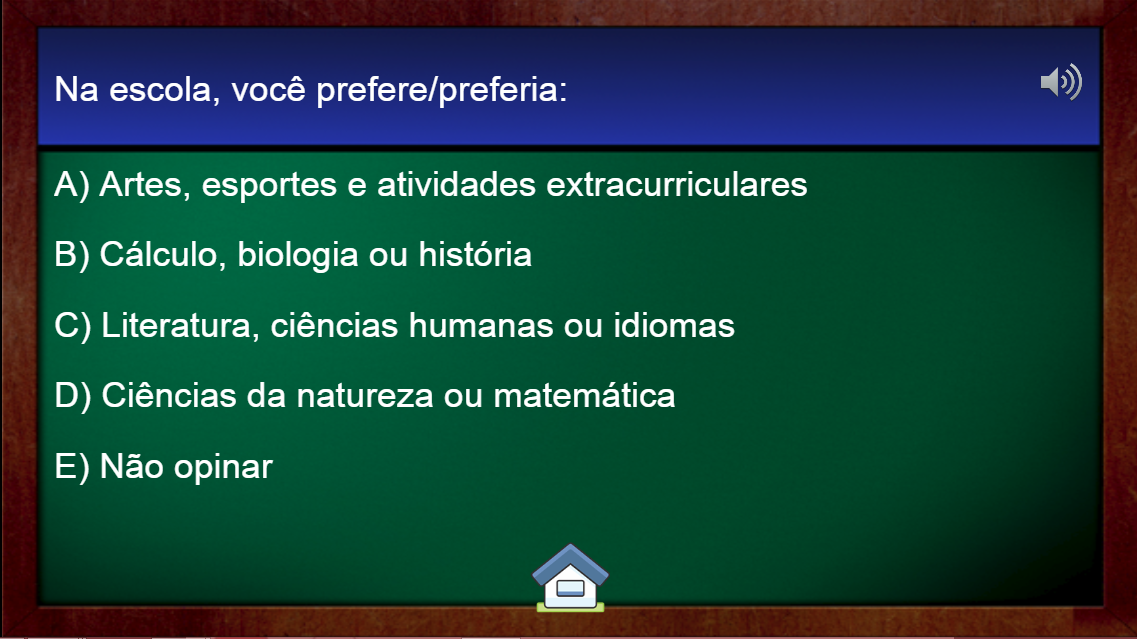
\includegraphics[width=0.95\textwidth]{Questionario.PNG} %% PARA COLOCAR O ARQUIVO DA IMAGEM NO SHARELATEX, CLIQUE NO ÍCONE QUE PARECE UMA FLECHINHA PARA CIMA (ATUALIZAR), CLIQUE EM UPLOAD E PROCURE A IMAGEM EM SEU COMPUTADOR.
\label{fig:testevocacional}
\end{figure}

O teste vocacional do aplicativo foi criado pela pedagoga e orientadora educacional Maria da Luz Calegari e traz uma orientação profissional baseada no temperamento das pessoas. “Desde 1999 é qualificada pela Coaching Psicologia Estratégica para aplicação e interpretação do MBTI®, instrumento que tem utilizado em trabalhos de aconselhamento vocacional e profissional.” \cite{maria}.

A pontuação é feita com um peso em cima de cada alternativa. Ao total são 25 questões com 5 alternativas em cada. Para cada alternativa que o usuário escolher, será acrescentado um ponto para aquela determinada letra correspondente, ao final das 25 questões foi feito a porcentagem de todas as alternativas baseando-se em quatro tipos de temperamentos disponibilizados pela autora do teste, que são eles: temperamento artesão, temperamento guardião, idealista e pensador intuitivo.

Logo em seguida, foi disponibilizado uma lista de cursos baseado na pontuação, sendo uma área de afinidade para cada alternativa e por fim, o discente poderá escolher um profissional dentre os listados. Na Figura \ref{fig:resultado} podemos observar algumas áreas de afinidade em que o usuário obteve maior pontuação.

\begin{figure} [H] 
\centering
%% hbt SIGNIFICA QUE ELE PRIMEIRO VAI TENTAR COLOCAR A IMAGEM NESTE LUGAR (h de "here"). SENÃO DER, ELE TENTA COLOCAR MAIS PRA BAIXO (b de "bottom"). SENÃO ELE COLOCA MAIS PARA CIMA (t de "top").

%% LABEL SERVE PARA VOCÊ REFERENCIAR A FIGURA NO MEIO DO TEXTO (VEJA LINHA 330: \ref{figura1}). ASSIM VOCÊ NÃO PERDE A REFERÊNCIA QUANDO MUDA A FIGURA DE LUGAR
\caption{Resultado: Lista de Cursos.}
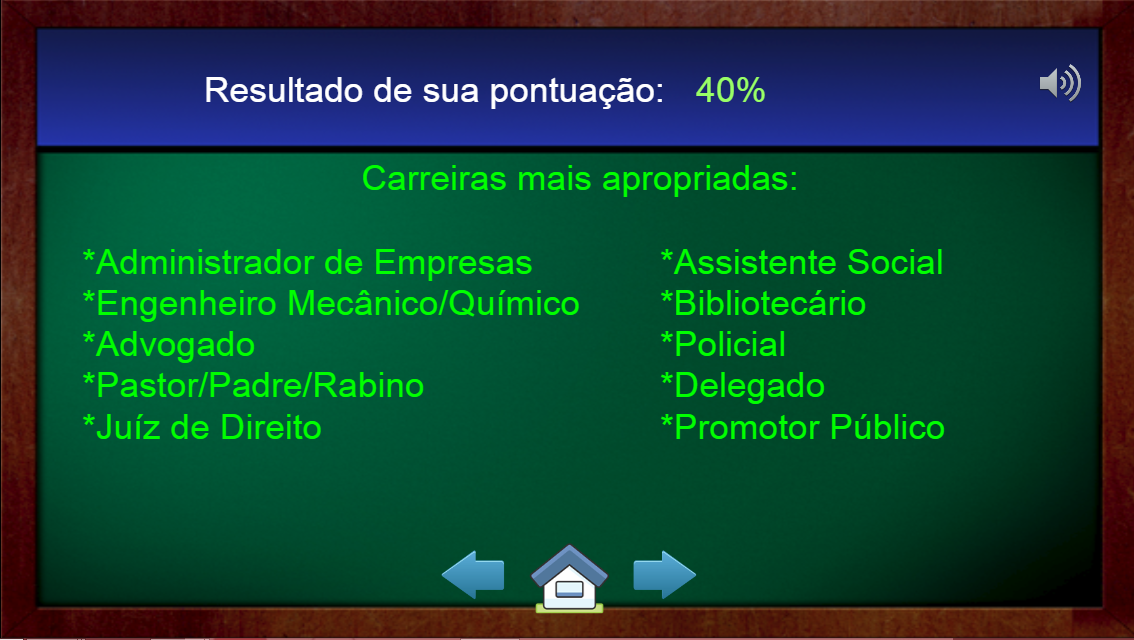
\includegraphics[width=0.95\textwidth]{Pontuacao.PNG} %% PARA COLOCAR O ARQUIVO DA IMAGEM NO SHARELATEX, CLIQUE NO ÍCONE QUE PARECE UMA FLECHINHA PARA CIMA (ATUALIZAR), CLIQUE EM UPLOAD E PROCURE A IMAGEM EM SEU COMPUTADOR.
\label{fig:resultado}
\end{figure}

Para a etapa das profissões foram implementadas apenas duas simulações virtuais, sendo elas: Professor e Médico. Na profissão do Professor, o participante dará aula sobre conhecimentos gerais. O foco desta etapa é apresentar este profissional em sala de aula. 

Ao final do conteúdo, o mesmo responderá a um breve questionário simulando uma prova. Na Figura \ref{fig:Norte}  podemos observar um pouco do conteúdo que é transmitido pelo professor e na Figura \ref{fig:Q2} podemos ver o questionário apresentado ao final do assunto ministrado pelo Professor.

\begin{figure}[H]
  \begin{subfigure}[b]{0.5\textwidth}
    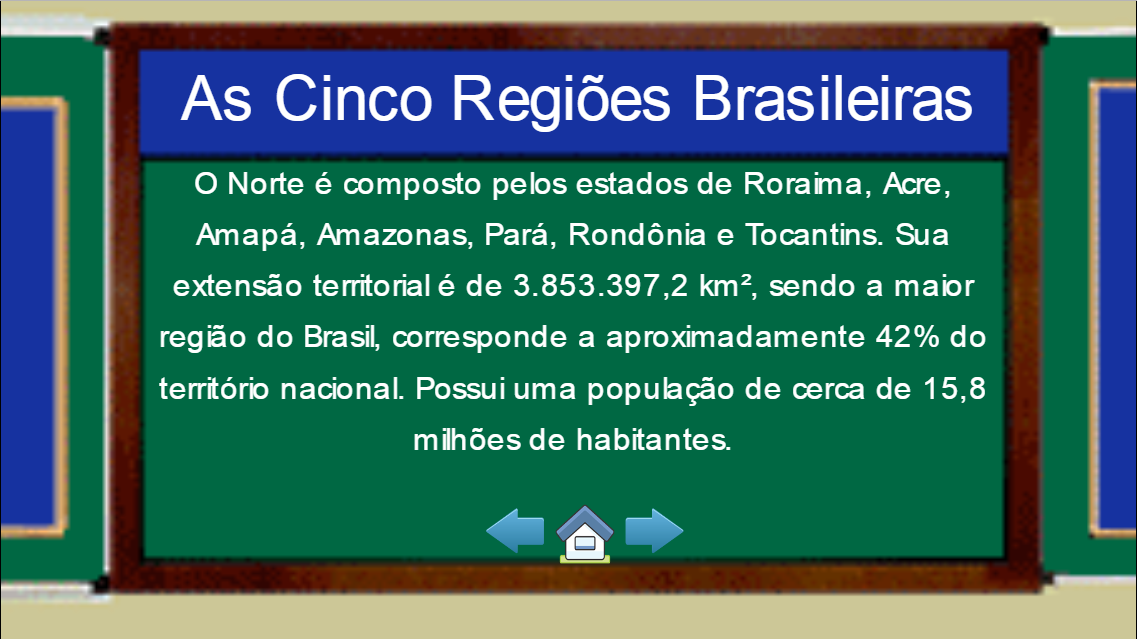
\includegraphics[width=\textwidth]{Norte.PNG}
    \caption{\textit{Conteúdo repassado pelo Professor}}
    \label{fig:Norte}
  \end{subfigure}
  \hfill
  \begin{subfigure}[b]{0.5\textwidth}
    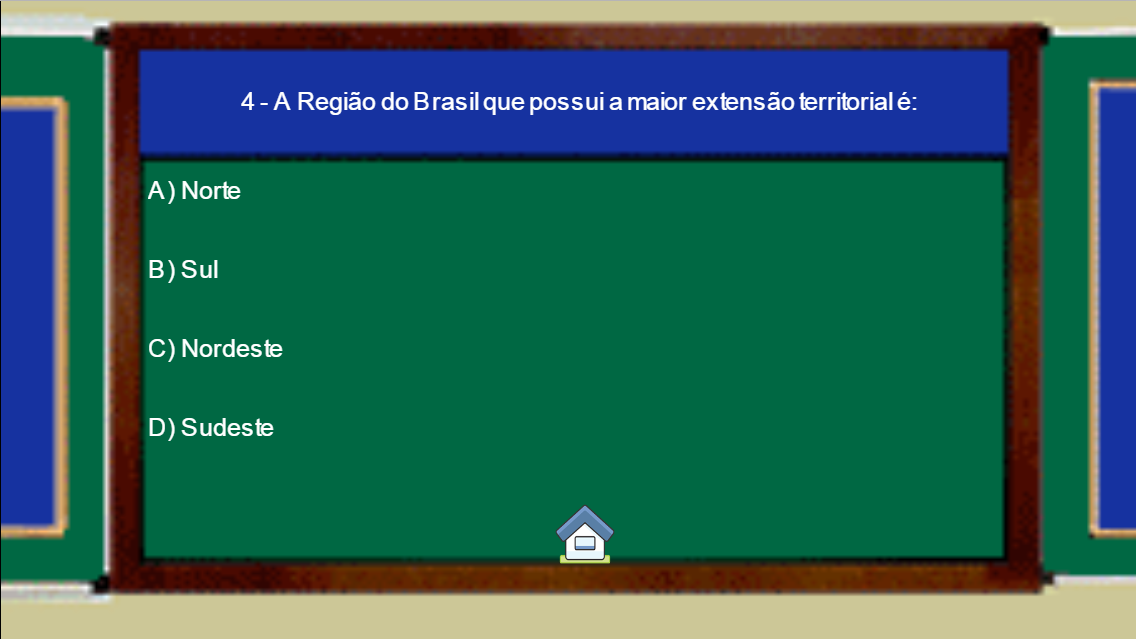
\includegraphics[width=\textwidth]{Q2.PNG}
    \caption{\textit{Questionário}}
    \label{fig:Q2}
  \end{subfigure}
  \caption{Simulação com o Professor.}
\end{figure}

O desenvolvimento da simulação do Médico foi feito por base no trabalho da \citeonline{francielli}, onde a mesma desenvolveu um simulador de cirurgia de Cataratas utilizando realidade virtual para que os profissionais da área pudessem fazer treinamentos. A técnica utilizada para a cirurgia foi a Facoemulsificação, sendo que todo o processo houve acompanhamento do Oftalmologista Dr. Carlos Roberto Gomes Fernandes.

Na simulação, o participante terá que acompanhar uma cirurgia de Cataratas. Para cada passo durante a operação, o mesmo receberá instruções do que deverá ser feito e de quais as ferramentas ele utilizará por vez, conduzindo cada uma delas até o local indicado, sendo que serão orientados em cada passo. Nas Figuras \ref{fig:f1} e \ref{fig:f2} podemos observar as instruções e ferramentas.

\begin{figure}[H]
  \begin{subfigure}[b]{0.5\textwidth}
    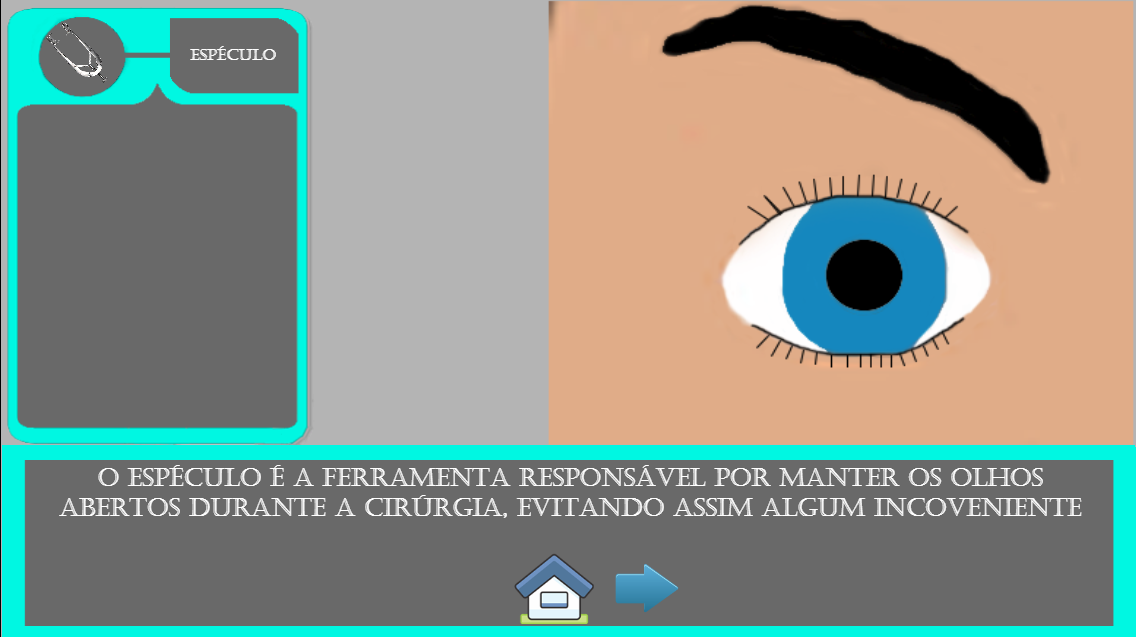
\includegraphics[width=\textwidth]{Medico1.PNG}
    \caption{\textit{Instruções}}
    \label{fig:f1}
  \end{subfigure}
  \hfill
  \begin{subfigure}[b]{0.5\textwidth}
    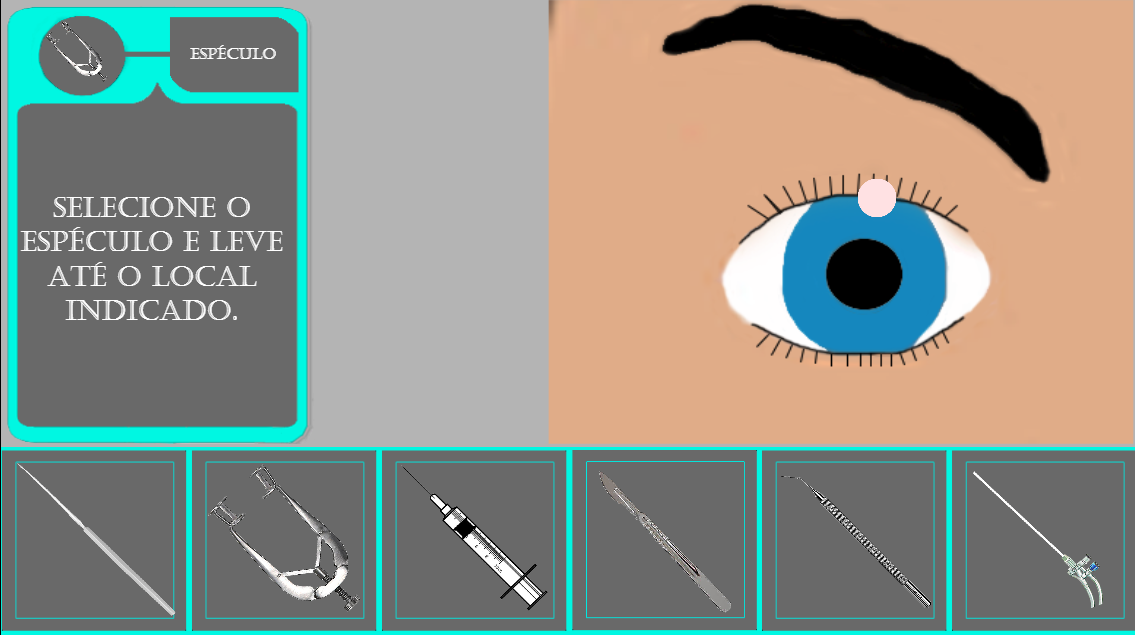
\includegraphics[width=\textwidth]{Medico2.PNG}
    \caption{\textit{Ferramentas}}
    \label{fig:f2}
  \end{subfigure}
  \caption{Simulação com o Médico.}
\end{figure}

\section{Ferramentas}

O \textit{framework} utilizado para o desenvolvimento do \textit{game} foi o \textit{Construct} 2\footnote{https://www.scirra.com/}: \textit{Software} criado pela \textit{Scirra} e lançado em 2011. Ferramenta de criação de jogos 2D que possui uma interação muito intuitiva e que pode ser usado em várias plataformas diferentes como \textit{Web} (HTML 5), \textit{Android}, \textit{Windows desktop}, dentre outras. O aplicativo é de fácil manipulação e o usuário não precisa ter muito conhecimento sobre desenvolvimento de jogos e programação de computador.

\chapter{Testes e Resultados}

Nesta seção serão abordados os testes e os resultados obtidos em uma pesquisa de campo com vinte e oito entrevistados, realizados em duas instituições de ensino público nas cidades de Picos na Unidade Escolar Jorge Leopoldo e em Colônia do Piauí no Ginásio Estadual Doutor José Gusmão.  

\section{Pesquisa de Campo}

Para a realização dos testes foi preparado um questionário com dez perguntas objetivas com o auxílio da Psicóloga Izabelly M. Costa do Nascimento da Universidade Federal do Piauí, referente ao perfil atual de cada entrevistado.

O objetivo do questionário é identificar o perfil de cada aluno, visando encontrar os meios de influências que envolvem os mesmos, as formas de Orientação Vocacional a que os mesmos recorreram e as profissões que os mesmos possuem afinidades caso tenham alguma.

O questionário foi disponibilizado ao final do jogo e durante a coleta de dados dos entrevistados, 18 dos 28 alunos afirmaram que intencionam seguir a carreira acadêmica após concluir o ensino médio, 3 deles pretendem trabalhar e 2 deles não souberam optar. Apesar de metade (14) dos alunos declararem que não sofrem influência alguma, 13 dos mesmos relatam que seus familiares são suas maiores influências, principalmente os pais.

Um outro dado importante foi à respeito do processo de orientação vocacional que eles haviam passado, onde apenas 2 deles fizeram apenas testes vocacionais \textit{online} sem terem nem um outro recurso para orientar-se.
No quesito profissional, 24 dos entrevistados responderam que já sabem que profissão pretendem seguir e dentre eles, 20 confirmaram que conhecem um pouco sobre o profissional.

Como resultado podemos observar que, apesar da maior parte dos discentes escolherem seguir a carreira acadêmica, os mesmos possuem um grande desafio que é a falta de orientação e a influência que recebem por parte dos seus familiares.

\section{Testes nas Instituições}

Para realizar os testes, os alunos foram organizados de forma individual para responderem primeiramente ao questionário disponibilizado no jogo. Após concluírem o teste, os mesmos verificaram a lista de curso fornecido de acordo com a afinidade de cada um, baseadas na escolha de suas alternativas.

Logo em seguida, para os discentes que obtiveram afinidade nas profissões de Medicina ou Professor iniciaram os testes envolvendo a simulação virtual, aos demais alunos puderam testar a fase prática sem que o resultado da coleta de dados durante a execução do jogo fosse alterado.

Ao finalizarem os testes, 20 dos 28 alunos afirmaram que se identificaram com alguma profissão dentre as listadas ao final do questionário e 18 dos que testaram a simulação virtual conseguiram encontrar afinidade no profissional. Sendo que os estudantes confirmaram que com a simulação virtual dos profissionais, eles puderam obter mais conhecimento sobre a área, além de contribuir mais para o momento de sua escolha.

Sobre as melhorias indicadas pelos estudantes estão o desenvolvimento de mais simulações virtuais dos profissionais e na formulação das perguntas e alternativas do questionário, deixando-as mais simples.

\section{Teste de Usabilidade}

Os testes de usabilidade foram feitos com onze alunos do Curso de Sistemas de Informação da Universidade Federal do Piauí - UFPI, sobre a Interação Humano Computador - IHC e com os 28 alunos entrevistados nas duas instituições. 

Segundo \citeonline{hix}, a usabilidade está diretamente relacionada com a \textit{interface}. \citeonline{Long} considera quatro parâmetros para medir a usabilidade que são: eficiência, aprendizagem, flexibilidade e atitude do utilizador.

Para as pesquisas foi utilizado a ferramenta ErgoList, que foi desenvolvido pelo Laboratório de Utilizabilidade da Informática - LabIUtil na Universidade Federal de Santa Catarina - UFSC, com o intuito de inspecionar a \textit{interface} permitindo ao estudante descobrir as falhas ergonômicas mais flagrantes em uma \textit{interface} com o usuário.

Na Figura \ref{fig:usabilidade} mostra um gráfico com as treze perguntas (Disponível nos Apêndices) em que os entrevistados responderam em relação aos testes de usabilidade. Observa-se que nas perguntas 2 e 8, referentes a ordem dos objetos no jogo e a linguagem em todas as etapas do jogo, foram onde se obteve maior pontuação.

Nota-se também que em nenhuma das perguntas se obteve maior pontuação negativa, exceto na pergunta 11, referentes aos erros apontados no jogo de forma negativa para o usuário, que as respostas coincidiram entre sim e não.

\begin{figure} [H] 
\centering
%% hbt SIGNIFICA QUE ELE PRIMEIRO VAI TENTAR COLOCAR A IMAGEM NESTE LUGAR (h de "here"). SENÃO DER, ELE TENTA COLOCAR MAIS PRA BAIXO (b de "bottom"). SENÃO ELE COLOCA MAIS PARA CIMA (t de "top").

%% LABEL SERVE PARA VOCÊ REFERENCIAR A FIGURA NO MEIO DO TEXTO (VEJA LINHA 330: \ref{figura1}). ASSIM VOCÊ NÃO PERDE A REFERÊNCIA QUANDO MUDA A FIGURA DE LUGAR
\caption{Resultado do Teste de Usabilidade.}
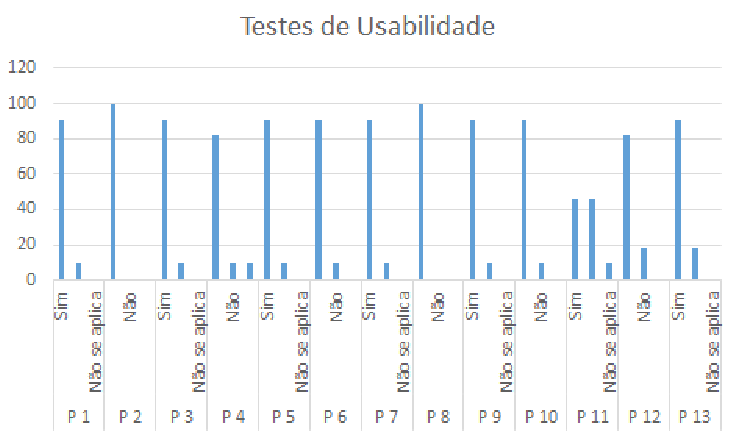
\includegraphics[width=0.90\textwidth]{usabilidade} %% PARA COLOCAR O ARQUIVO DA IMAGEM NO SHARELATEX, CLIQUE NO ÍCONE QUE PARECE UMA FLECHINHA PARA CIMA (ATUALIZAR), CLIQUE EM UPLOAD E PROCURE A IMAGEM EM SEU COMPUTADOR.
\label{fig:usabilidade}
\end{figure}


% ---
% Conclusão
% ---
\chapter{Considerações Finais}

De acordo com o exposto, observa-se que o projeto proposto foi de grande relevância pois alcançou os resultados esperados, que foi a interação do discente com a simulação dos profissionais disponibilizados no \textit{game}, permitindo-os ter o conhecimento e entendimento sobre sobre determinadas profissões contribuindo assim para sua maturação ou escolha vocacional. 
 
Podemos perceber que quanto mais conteúdos for disponibilizado ao aluno, mais chances o mesmo terá de formular suas próprias conclusões. A simulação das profissões integradas ao questionário serviram como base para identificar seu perfil profissional.

Embora nem todos os discentes puderam se identificar com o profissional indicado ao final do teste, podemos observar que para a maior parte deles o jogo foi fundamental na busca de sua área profissional e na identificação do seu perfil (autoconhecimento). 

\section{Trabalhos Futuros}

Propõe-se como projetos futuros o desenvolvimento de novas simulações virtuais de alguns profissionais, para que os usuários possam ter mais opções durante a escolha de um perfil profissional. Além da integração do projeto proposto nas mais diversas plataformas, possibilitando aos utilizadores terem acesso ao \textit{software} em locais inacessíveis a computadores ou \textit{internet}. 


% ----------------------------------------------------------
% ELEMENTOS PÓS-TEXTUAIS
% ----------------------------------------------------------
\postextual


% ----------------------------------------------------------
% Referências bibliográficas
% ----------------------------------------------------------
\bibliography{references} %% REFERENCIA AO ARQUIVO abntex2-modelo-references.bib

% ----------------------------------------------------------
% Glossário
% ----------------------------------------------------------
%
% Consulte o manual da classe abntex2 para orientações sobre o glossário.
%
%\glossary

% ----------------------------------------------------------
% Apêndices
% ----------------------------------------------------------

% ---
% Inicia os apêndices
% ---
\begin{apendicesenv}

% Imprime uma página indicando o início dos apêndices
\partapendices

\chapter{Apêndice}

\vspace{-2cm} 

\begin{center}
\begin{longtable}{l|l}
\caption{Teste Vocacional.} 
\label{tab:questionario}
\columnsep=5cm

\cr \hline \multicolumn{1}{|c|}{\textbf{Perguntas}} & \multicolumn{1}{c|}{\textbf{Alternativas}} 
\endfirsthead

\multicolumn{3}{c}{{\bfseries \tablename \thetable{} -- Continuação da tabela anterior}} \\ 
\cr \hline \multicolumn{1}{|c|}{\textbf{Perguntas}} &
\multicolumn{1}{c|}{\textbf{Alternativas}} \\ \hline 
\endhead

\hline \multicolumn{3}{l}{{Continua na próxima página}} \\ \hline
\endfoot

\hline \hline
\endlastfoot
    \hline
    Na escola, você prefere/preferia & a) Arte, esportes ou atividades \\ & extracurriculares \\ & b) Cálculo, biologia ou história\\ & c) Literatura, ciências humanas ou \\ & idiomas\\ & d) Ciências da natureza ou \\ & matemática \\ & e) Não opinar
    \cr \hline 
    Quais assuntos você costuma ler com mais \\ frequência & a) Política/Políticas Publicas\\ & b) Educação ou tratamento de \\ & doenças\\ & c) Economia ou problemas sociais\\ & d) Ciências e Tecnologia\\ & e) Não opinar 
    \\ \hline
    Você se descreveria como uma pessoa & a) Impulsiva e um tanto aventureira\\ & b) Cuidadosa e sempre responsável \\ & c) Entusiasmada e muito amiga\\ & d) Calma e diferente da maioria\\ & e) Não opinar
    \\ \hline
    Você se considera uma pessoa & a) Prática e hábil para improvisar\\ & b) Batalhadora, que sabe o que quer\\ & c) Preocupada com questões \\ & humanas\\ & d) Capacitada para criar e inventar\\ & e) Não opinar
    \\ \hline
    De quais características sua você sente orgulho & a) Coragem e facilidade para lidar \\ & com o inesperado\\ & b) Senso de dever e capacidade \\ & de dar exemplo\\ & c) Idealismo e talento para \\ & compreender os outros\\ & d) Engenhosidade e capacidade \\ & mental\\ & e) Não opinar
    \\ \hline
    Costuma confiar mais em & a) Impulsos e instintos \\ & b) Costumes e tradições\\ & c) Pressentimentos e palpites\\ & d) Razão e lógica\\ & e) Não opinar        \\ \hline
    Quando conhece uma pessoa interessante, você & a) Se comunica logo e até faz \\ & amizade\\ & b) Avalia, antes, sua origem\\ & c) Se comunica, mas evita a \\ & proximidade\\ & d) Espera que ela se apresente\\ & e) Não opinar
    \\ \hline
    Quase sempre, você gosta de & a) Causar impacto: os holofotes o/a \\ & atraem \\ & b) Ser visto como membro valioso \\ & de um grupo\\ & c) Sonhar em transformar o mundo, \\ & para melhor\\ & d) Desvendar um enigma ou inventar \\ & algo útil\\ & e) Não opinar
    \\ \hline
    A vida é mais interessante quando se tem & a) Desafios, situações que mudam,\\ & adrenalina\\ & b) Segurança, emprego garantido,\\ & integração social\\ & c) Possibilidade de fazer algo em \\ & favor das pessoas\\ & d) Possibilidade de ir além do \\ & que já é conhecido\\ & e) Não opinar
    \\ \hline
    Você gosta de ser lembrado por & a) Sua alegria, bondade e \\ & espontaneidade\\ & b) Seu comprometimento com o \\ & que é considerado certo\\ & c) Seu modo compreensivo e \\ & tolerante\\ & d) Seu jeito autônomo de tocar \\ & a vida\\ & e) Não opinar
    \\ \hline
    Você gostaria de ser um & a) Craque na profissão que escolher\\ & b) Executivo bem-sucedido\\ & c) Profissional reconhecido pela \\ & ética\\ & d) Especialista ou cientista\\ & e) Não opinar
    \\ \hline
    Você é muito bom (boa) lidando com & a) Ferramentas, instrumentos e \\ &equipamentos\\ & b) Controle do tempo, comando e \\ &execução\\ & c) Pessoas de todos os níveis \\ & culturais e sociais\\ & d) Sistemas e construção \\ & (material ou mental)\\ & e) Não opinar
    \\ \hline
    Antes de agir, você analisa as & a) Vantagens imediatas\\ & b) Experiências já vividas\\ & c) Possibilidades futuras\\ & d) Condições e consequências\\ & e) Não opinar
    \\ \hline
    Gosta quando as pessoas & a) O surpreendem com um elogio\\ & b) Acatam seus conselhos/suas \\ & orientações\\ & c) Reconhecem sua integridade e\\ & singularidade\\ & d) Reconhecem sua inteligência\\ & e) Não opinar
    \\ \hline
    Você costuma abraçar um novo projeto & a) Com a cara e a coragem\\ & b) Guiado pela experiência\\ & c) Confiando na intuição e na \\ & criatividade\\ & d) Depois de verificar todas as \\ & variáveis\\ & e) Não opinar
    \\ \hline
    Você acha que precisaria ser mais & a) Paciente\\ & b) Relaxado\\ & c) Esperto\\ & d) Sociável\\ & e) Não opinar                                \\ \hline
    Geralmente, você prefere agir & a) No calor do momento\\ & b) Com segurança e conforme o \\ & costume\\ & c) Quando está inspirado\\ & d) Quando um enigma o/a desafia\\ & e) Não opinar                                  \\ \hline
    Se sente motivado quando & a) As coisas mudam continuamente\\ & b) Sabe em que terreno (firme) está \\ & pisando\\ & c) Harmonia e inspiração guiam a \\ & atividade\\ & d) Há liberdade para projetar o \\ & futuro\\ & e) Não opinar
    \\ \hline
    Em atividades de grupo, você prefere & a) As imprevisíveis, que exigem ação \\ & rápida\\ & b) Administrar os meios e recursos\\ & disponíveis\\ & c) Motivar as pessoas para darem o \\ & melhor\\ & d) Descartar logo o que não funciona\\ & e) Não opinar
    \\ \hline
    Em relação à vida, você acha que se sai melhor \\ quem & a) Vive simplesmente: deixa rolar...\\ & b) Trabalha duro, pois viver é lutar\\ & c) Nunca deixa de sonhar e corre \\ & atrás do sonho\\ & d) Procura entender eventos e \\ & fenômenos\\ & e) Não opinar
    \\ \hline
    Você vai ao culto religioso & a) Para encontrar amigos/paquerar\\ &  b) Para cumprir um preceito familiar\\ & c) Para buscar harmonização interior\\ & d) Somente em situações especiais\\ & e) Não opinar
    \\ \hline
    Liderar é uma atividade que gosta de exercer & a) Por pouco tempo (depende da \\ & situação)\\ & b) Quando pode comandar do começo \\ & ao fim\\ & c) Quando é preciso identificar e \\ & reunir\\ & talentos\\ & d) Quando pensamento estratégico é\\ & necessário\\ & e) Não opinar
    \\ \hline
    Em uma escola, você gostaria de ser & a) Professor de artes/ educação física\\ & b) Diretor\\ & c) Orientador educacional ou \\ & pedagógico\\ & d) Professor de matemática/química \\ & ou física\\ & e) Não opinar
    \\ \hline
    É um elogio quando se referem a você como & a) Corajoso, otimista e divertido\\ & b) Cauteloso, responsável e aplicado\\ & c) Harmonizador, íntegro e culto\\ & d) Uma pessoa com mente brilhante\\ & e) Não opinar
    \\ \hline
    Frases que têm a ver com você & a) “Viver e não ter a vergonha de \\ & ser feliz...”\\ & b) “Manda quem pode; obedece \\ & quem tem juízo”\\ & c) “Para seu próprio interesse, seja\\ & verdadeiro”\\ & d) “Penso, logo existo”\\ & e) Não opinar
    \\ \hline
\end{longtable}
\end{center}



\begin{center}
\begin{longtable}{l|l}
\caption{Perguntas retiradas da Ferramenta ErgoList.} 
\label{tab:ErgoList}
\columnsep=5cm

\cr \hline 
\multicolumn{1}{|c|}{\textbf{Perguntas}} & \multicolumn{1}{c|}{\textbf{Alternativas}} 
\endfirsthead

\multicolumn{3}{c}%
{{\bfseries \tablename\ \thetable{} -- Continuação da tabela anterior}} \\ 
\hline \multicolumn{1}{|c|}{\textbf{Perguntas}} &
\multicolumn{1}{c|}{\textbf{Alternativas}} \\ \hline 
\endhead

\hline \multicolumn{3}{l}{{Continua na próxima página}} \\ \hline
\endfoot

\hline \hline
\endlastfoot
    \hline
    As páginas possuem denominações de menus de acordo com o que \\ eles representam? & [  ] Sim \\ & [  ] Não \\ & [  ] Não se aplica
    \\
    \hline
    A disposição dos objetos seguem uma ordem lógica? & [  ] Sim \\ & [  ] Não \\ & [  ] Não se aplica
    \\
    \hline
    O sistema fornece \textit{feedback} para todas as ações do usuário? & [  ] Sim \\ & [  ] Não \\ & [  ] Não se aplica
    \\
    \hline
    As denominações dos itens são breves? & [  ] Sim \\ & [ ] Não \\ & [  ] Não se aplica
    \\
    \hline
    A navegação pelo \textit{software} é fácil? & [  ] Sim \\ & [ ] Não \\ & [  ] Não se aplica
    \\
    \hline
    O \textit{software} proporciona a interação entre Aprendiz X Agente de \\ Aprendizagem? & [  ] Sim \\ & [ ] Não \\ & [  ] Não se aplica
    \\
    \hline
    A \textit{interface} é amigável? & [  ] Sim \\ & [ ] Não \\ & [  ] Não se aplica
    \\
    \hline
    As mensagens e textos das interfaces apresentam-se em língua \\ portuguesa? & [  ] Sim \\ & [ ] Não \\ & [  ] Não se aplica
    \\
    \hline
    É fácil de aprender e usar? & [  ] Sim \\ & [ ] Não \\ & [  ] Não se aplica
    \\
    \hline
    Você considera o \textit{software} útil? & [  ] Sim \\ & [ ] Não \\ & [  ] Não se aplica
    \\
    \hline
    O erro é apontado ao aluno no software como algo negativo? & [  ] Sim \\ & [ ] Não \\ & [  ] Não se aplica
    \\
    \hline
    Os contextos são adequados e atraentes? (\textit{interface}) & [  ] Sim \\ & [ ] Não \\ & [  ] Não se aplica
    \\
    \hline
    A linguagem utilizada é apropriada e de fácil entendimento? & [  ] Sim \\ & [ ] Não \\ & [  ] Não se aplica
    \\
    \hline
\end{longtable}
\end{center}

\end{apendicesenv}
% ---
\end{document}
